\section{Model Comparison}\label{sec:comparisons}

The fundamental problem in comparing Sgr A* models to the data is variability.  We do not expect even an ideal numerical evolution of a source model to match the data point for point, because the space of possible realizations of the model is very large.  But we do expect the {\em distribution} of observables to match an accurate model.  For example, we might expect that the observed 86 GHz flux $F_{86}$ is consistent with being drawn from the distribution of 86GHz fluxes from the model.

Since most observables are correlated over some time $\tau \sim $few $\times 100 G M/c^3$, to obtain the mean and variance of the model distribution to accuracy $f$ we would need a simulation of duration $\sim \tau/f^2 \sim 30,000 (\tau/300) (f/0.1)^{-2}$.  This requires between $10^3$ and $10^4$ node-hours on a state of the art cluster node, depending on the desired resolution, duration, and code used.  This is expensive since $\sim 10$ runs are used for each model set, and runs frequently need to be repeated for multiple values of the numerical parameters (e.g. resolution).  Most of the models used here have been run for either $10,000$ or $30,000 \tg$, although a few have been run to $100,000 \tg$.

The constraints are heterogeneous in the sense that some are related to time-averaged non-contemporaneous measurements (e.g. the NIR flux constraint), while others are instantaneous values measured during the EHT observing campaign (e.g. the m-ring fits), so it is impossible at present to use a single technique to estimate $p$ values for all constraints.

In what follows we will look at each constraint independently (i.e. we will ignore correlations) and generate a $p$ value.  We then cut models with $p < 0.01$.

[CG, Michi to write]

%==============================================================================
\subsection{Thermal, Aligned Models}

Illinois, Frankfurt, HAMR, critical beta thermal models

%------------------------------------------------------------------------------
\subsubsection{EHT Constraints}

First we compare data and models using the VLBI null location statistic, the pre-image size, and the ring diameter, ring thickness, and ring asymmetry from m-ring fitting.

It turns out that the null location statistic is informative and tends to rule out edge-on models when $R_{high} > 1$.  The pre-image size statistic is simple but not powerful: most of the models are about the right size, and only a very few face-on, low $R_{high}$ models are too large.   The m-ring fitting is highly informative.  Many of our thermal models look like the data, but - for example - edge on MAD models are large values of $R_{high}$ and positive spin are strongly disfavored because they are too asymmetric.

%..............................................................................
\subsubsubsection{Null Location}

[CK to summarize]

% Statement about consistency between overlapping model sets.

\begin{figure*}
  \centering
  [altex]
  \caption{The left panels show two snapshots from a GRMHD simulation
    with SANE field configuration and black hole spin $a=0.5$ and the
    right panels the corresponding visibility amplitudes for a
    horizontal and a vertical cross section through the images.
    The snapshot in the top row obeys both selection criteria: the
    minima are in the 2.5-3.5 G$\lambda$ range and the amplitude in
    the $6-8$G$\lambda$ is below 6\%.
    The image in the bottom row, on the other hand, is an example that
    has no minimum in one cross section and too much power at long
    baselines, due to the asymmetry introduced by a transient bright
    structure in the flow.}
  \label{fig:cmp_VA}
\end{figure*}

\begin{figure}
  \centering
  [altex]
  \caption{Visibility amplitude as a function of baseline length
    observed on 2017 April 7.
    The pink band marks the location of the first minima in the
    visibility amplitude along different orientations.
    The horizontal red line marks our conservative upper limit for the
    observed visibility amplitude between $6-8$G$\lambda$.}
  \label{fig:cmp_null}
\end{figure}

\begin{figure}
  \centering
  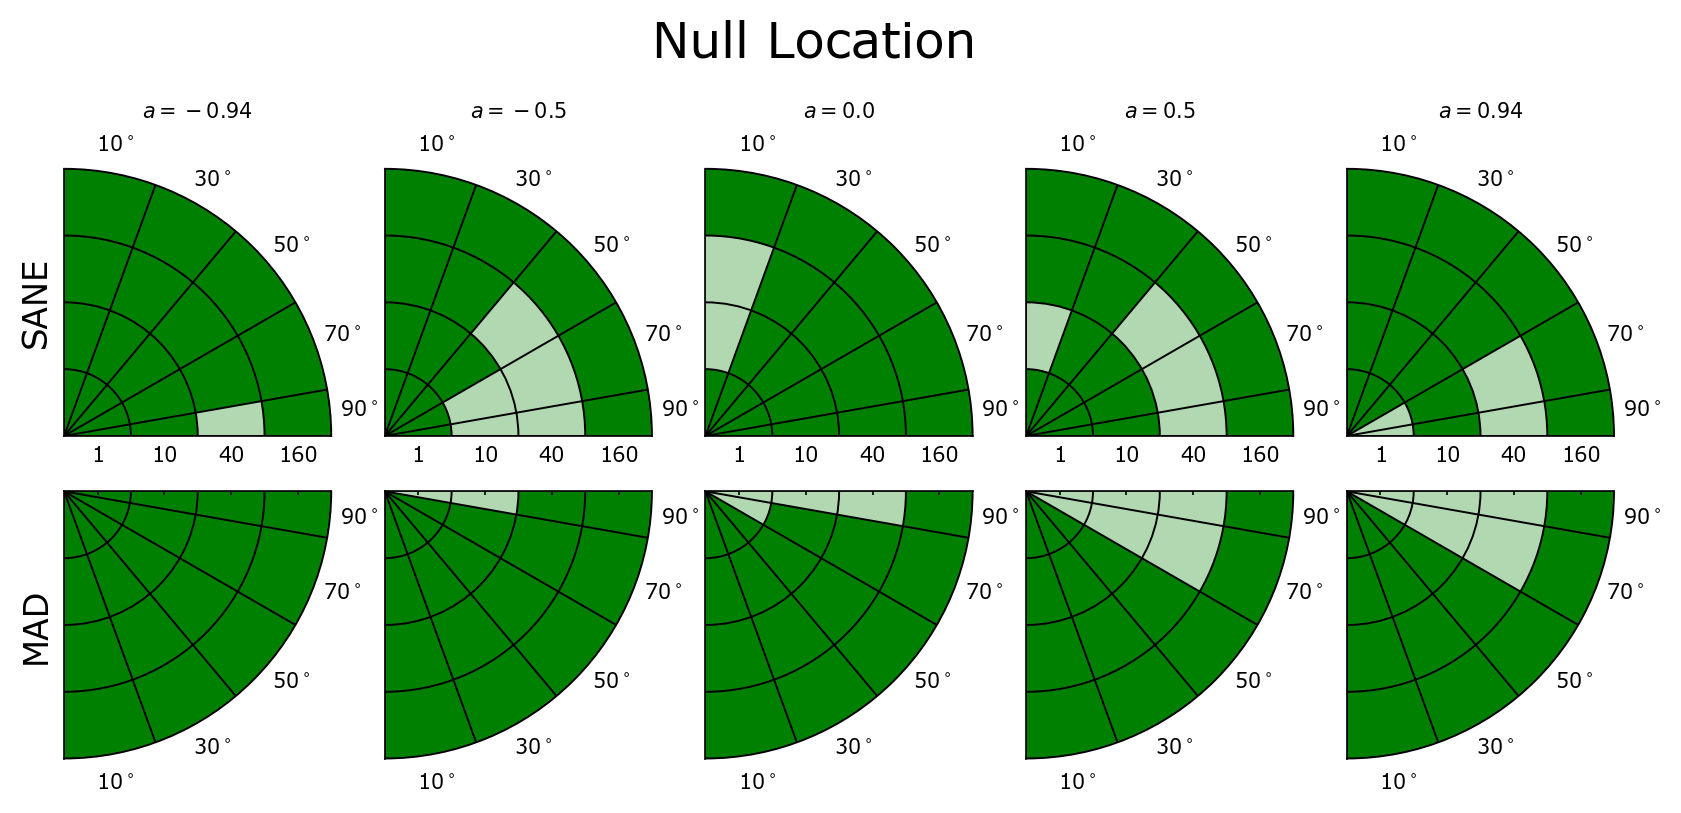
\includegraphics[width=\columnwidth]{./figures/Ozel.png}
  \caption{Ozel constraints plots}
  \label{fig:cmp_ozel}
\end{figure}

...

%..............................................................................
\subsubsubsection{Pre-imaging Size}

\begin{figure}
  \centering
  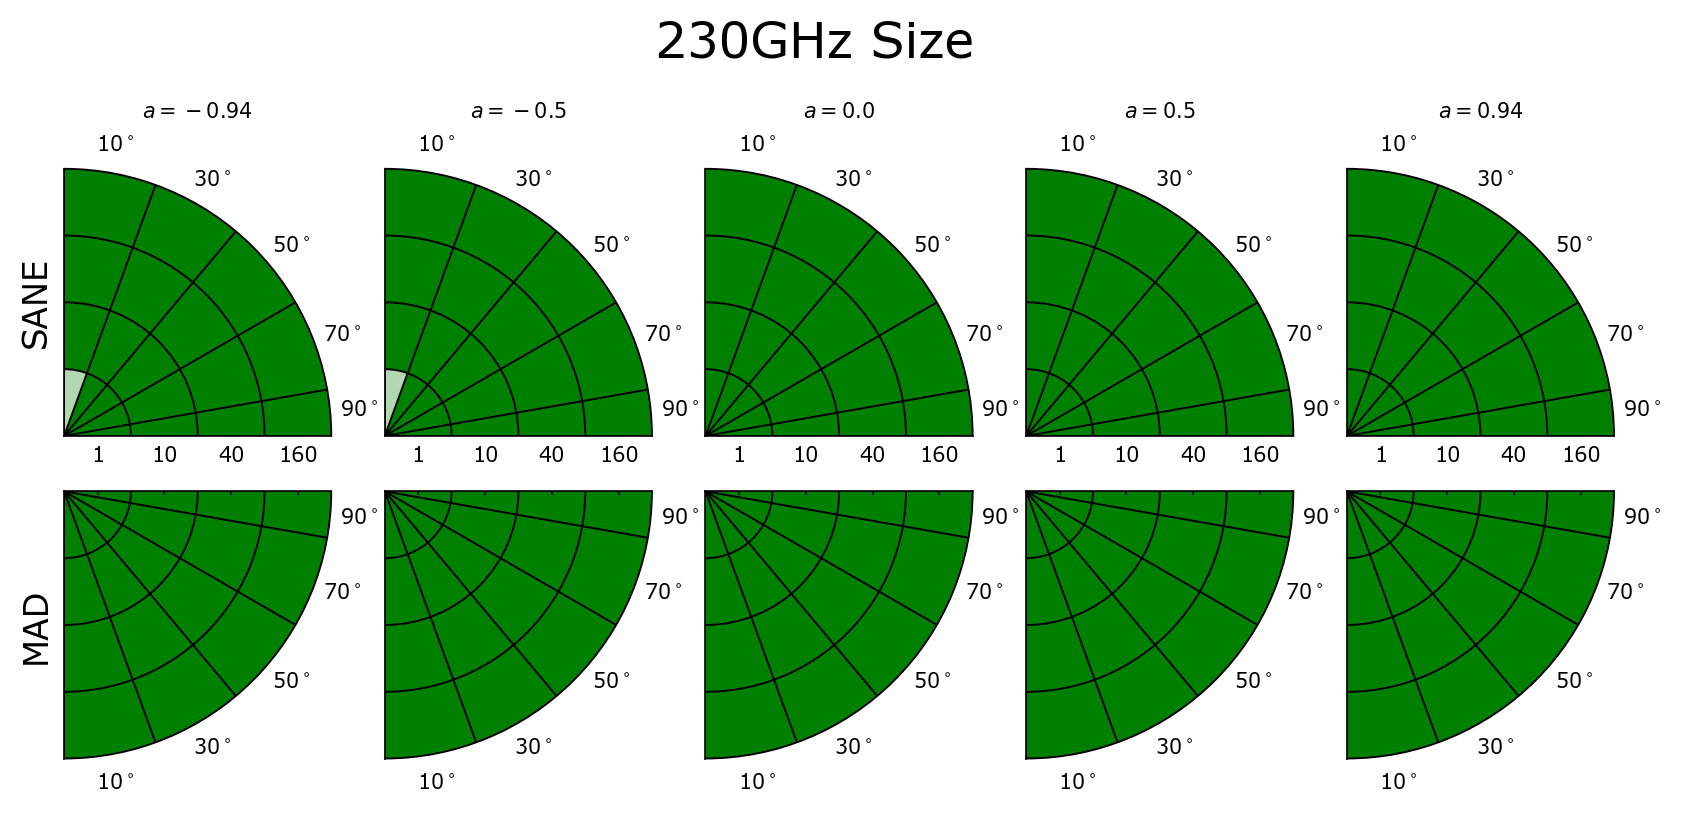
\includegraphics[width=\columnwidth]{./figures/230GHz_size.png}
  \caption{2nd moment plots}
  \label{fig:cmp_2nd_moment}
\end{figure}

[Andrew to summarize]

%..............................................................................
\subsubsubsection{M-ring Fits}

Diameter, Width, and Asymmetry of M-rings.

Michi

\begin{figure}
  \centering
  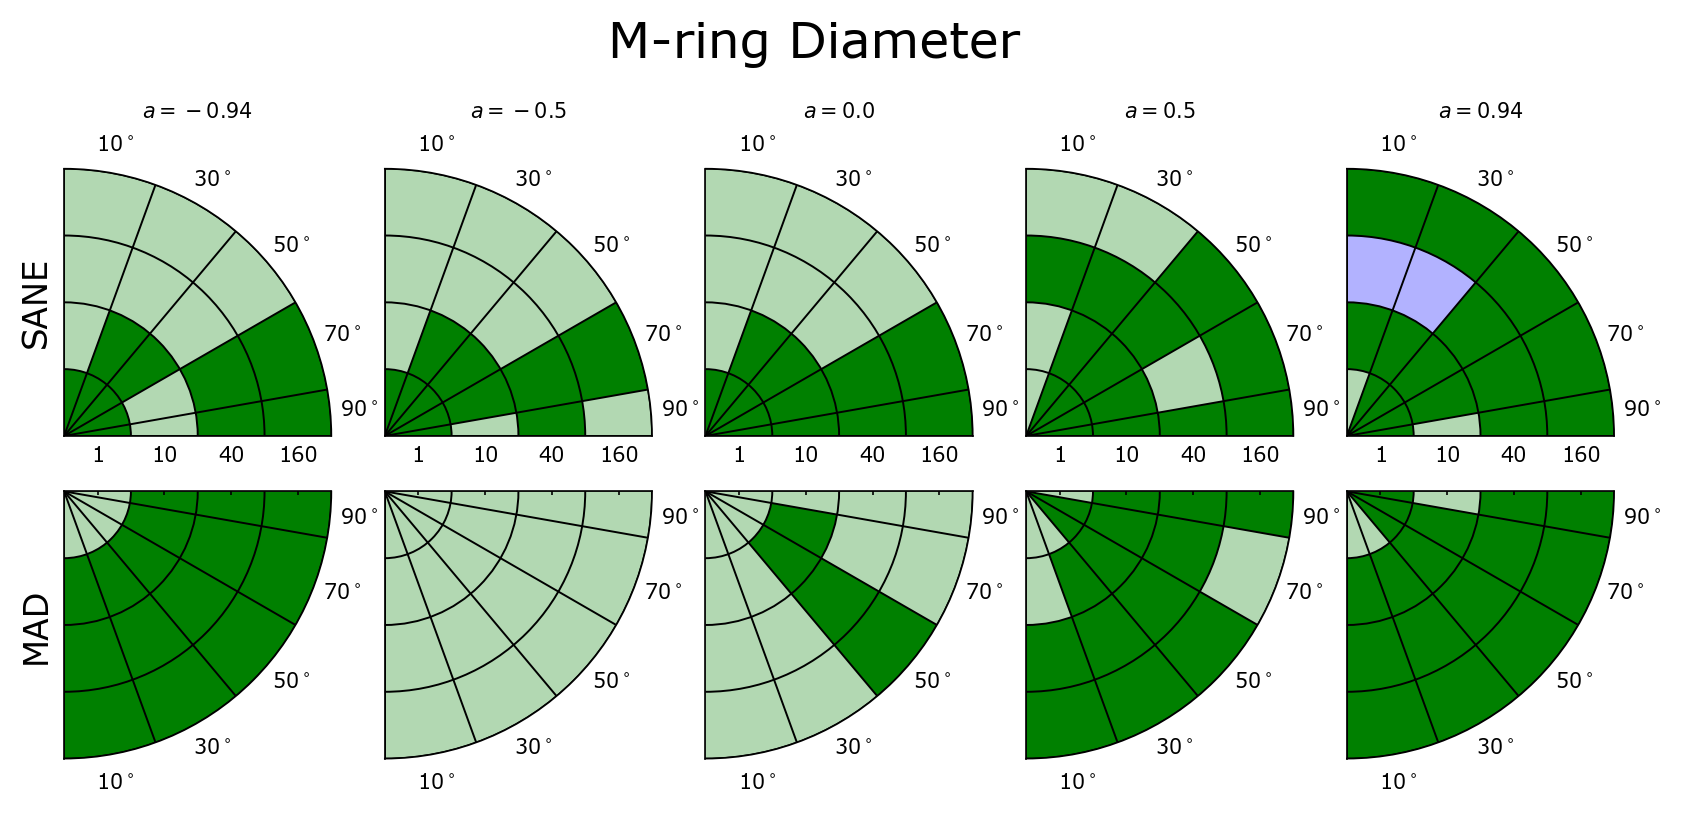
\includegraphics[width=\columnwidth]{./figures/r0.png}
  \caption{M-Ring diameter.}
  \label{fig:cmp_m-ring_diam}
\end{figure}
\begin{figure}
  \centering
  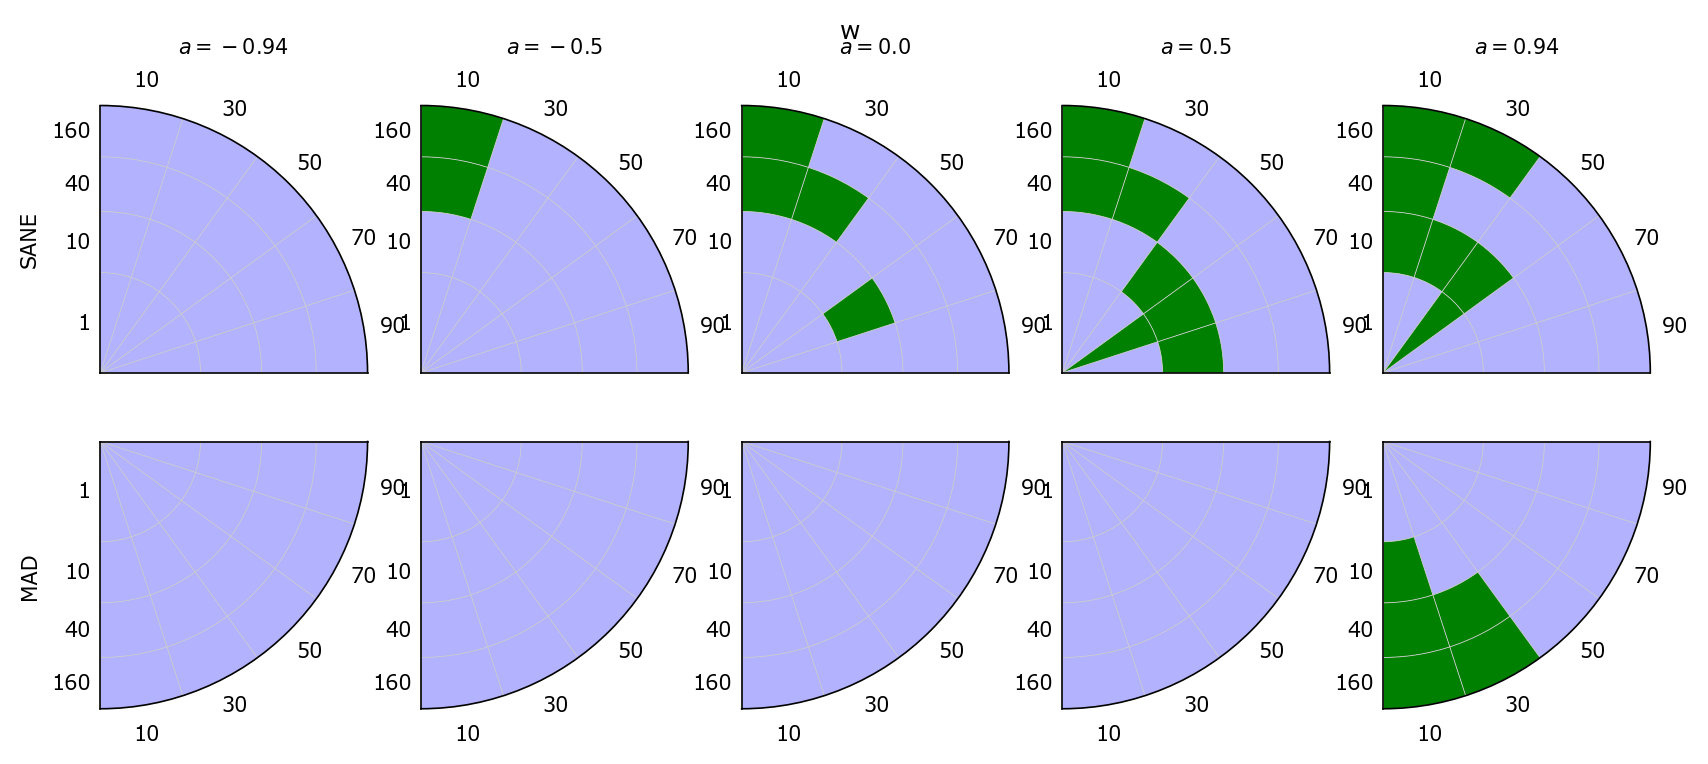
\includegraphics[width=\columnwidth]{./figures/w.png}
  \caption{m-ring widths}
  \label{fig:cmp_m-ring_width}
\end{figure}
\begin{figure}
  \centering
  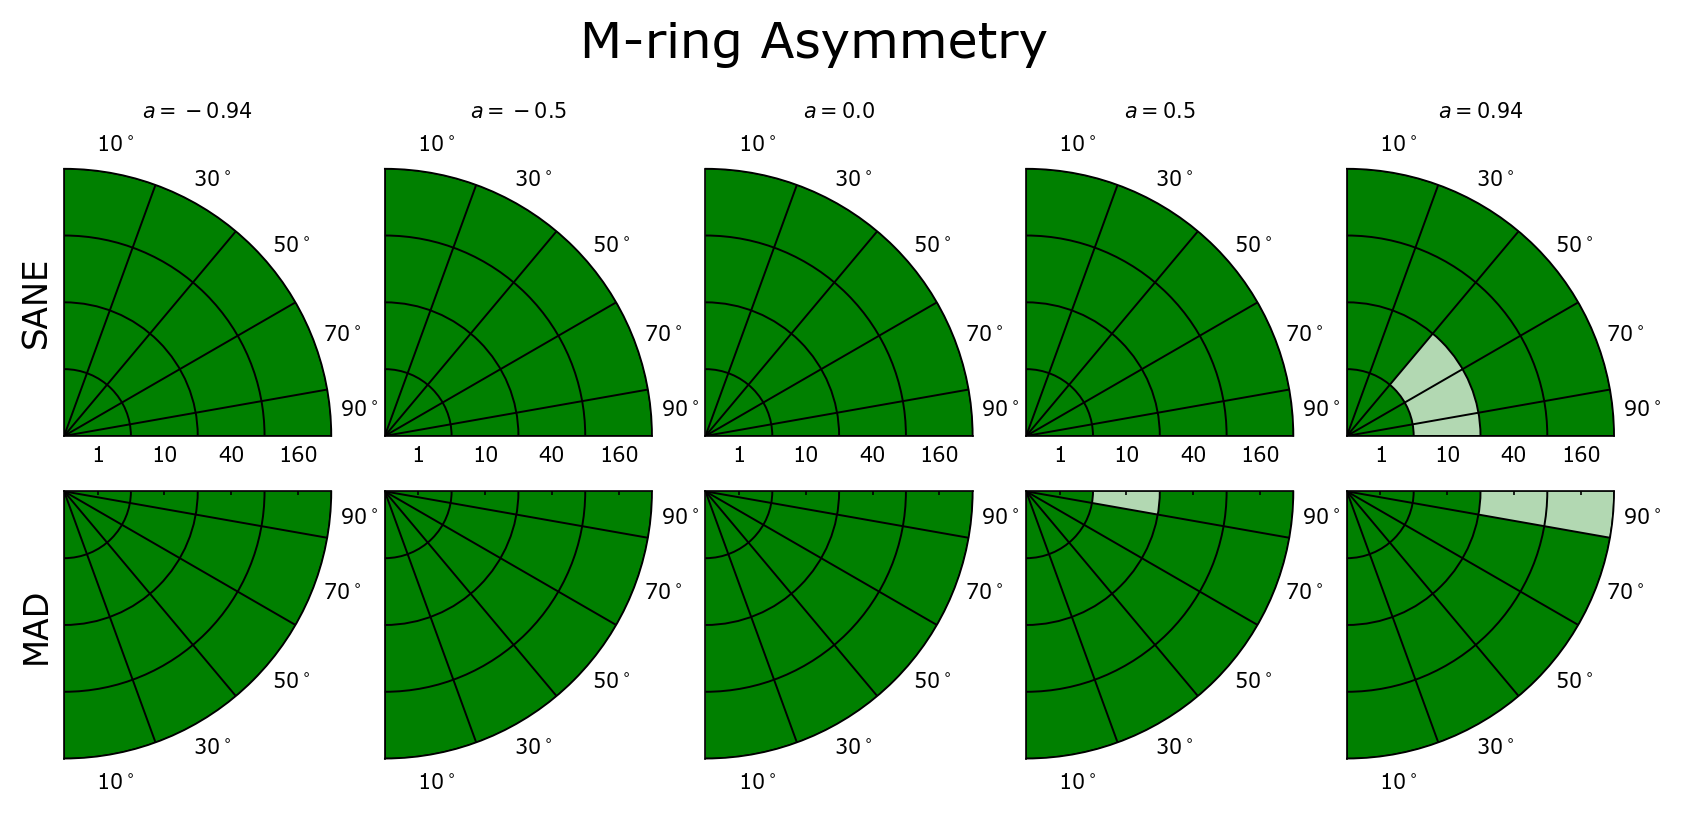
\includegraphics[width=\columnwidth]{./figures/f1.png}
  \caption{m-ring asymmetry}
  \label{fig:cmp_m-ring_asymm}
\end{figure}

\subsubsubsection{EHT Constraint Summary}

\begin{figure}
  \centering
    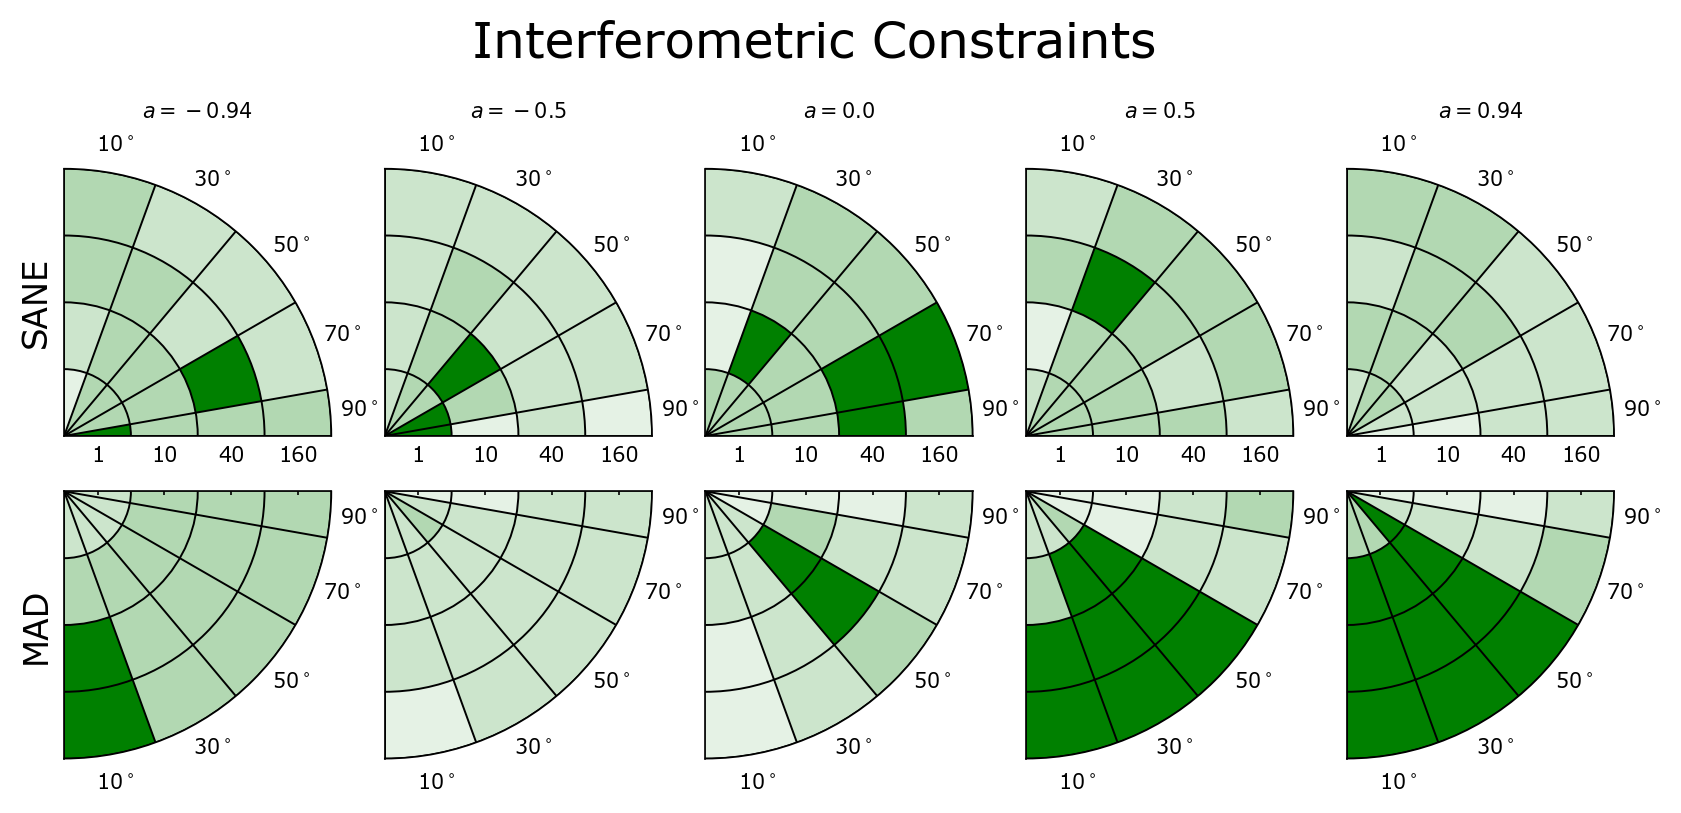
\includegraphics[width=\columnwidth]{./figures/Interferometric_Hard_Cut.png}
  \caption{Combined interferometric constraints (logical {\em and}) including the second moment, null location, and m-ring fit constraints.}
  \label{fig:all_EHT_constraints}
\end{figure}

%------------------------------------------------------------------------------
\subsubsection{Variability}

Variability is central to interpretation of Sgr A*: the small black hole size means that observations considered here are taken over intervals when the source is expected to vary significantly.  This distinguished Sgr A* from M87*, where the source is expected to vary only over timescales long compared to a single track.

Variability is a strong constraint on the models.  Although models differ in their degree of variability, both in an integrated sense and on 4 $G\lambda$ baselines, only a very small fraction of models are as quiet as the data (these tend to be face-on SANE models).  This is true whether we use data from one day, all days, or include measurements of light curve variability from historical monitoring of Sgr A*.   In general, SANE models are quieter than MAD models, and (less strongly) face-on models are quieter than edge-on models.

If we were to apply the variability constraints directly to the models there would be M/N successful models left (M1/N for the ALMA constraint and M2/N for the visibility amplitude constraint).  One interpretation of this result is that the surviving models are the correct description of the source (although we would expect some misclassification of models as consistent or inconsistent when using 1\% cuts on such a large model set).  Another interpretation is that there is a missing physical ingredient in the models, see Section \ref{sec:discussions} for a discussion.

%..............................................................................
\subsubsubsection{ALMA Light Curve}

\begin{figure}
  \centering
    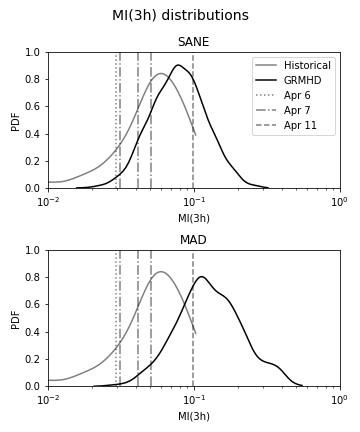
\includegraphics[width=\columnwidth]{./figures/mi_dist.png}
  \caption{Distributions of MI for Illinois thermal models, compared to distributions from historical observations and the values from the 2017 ALMA light curve. }
  \label{fig:cmp_ALMA_var}
\end{figure}

[David Lee to provide first draft]

%..............................................................................
\subsubsubsection{4 $G\lambda$ Visibility Amplitude Variability}

\begin{figure}
  \centering
    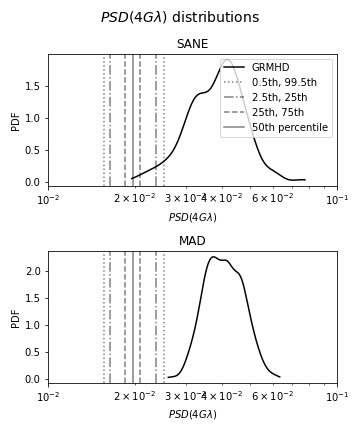
\includegraphics[width=\columnwidth]{./figures/va_dist.png}
  \caption{Distributions of $PSD(4G\lambda)$ for Illinois thermal models, compared to the observed value from the 2017 EHT campaign. }
  \label{fig:cmp_VLBI_var}
\end{figure}

[Boris to provide first draft]

%------------------------------------------------------------------------------
\subsubsection{Non-EHT Constraints}

Here we compare constraints from 86GHz, NIR, and X-ray observations.  Emission in these bands is believed to originate in the compact source from plasma that is close to or overlaps the plasma that produces the 230GHz emission observed by EHT.

It turns out that the 86GHz flux and size do not discriminate strongly between models: most models have about the right size and spectral index.  The NIR and X-ray constraints - which require that our models not overproduce the observed emission - are highly informative.  It turns out that many SANE models with large $\Rh$ (and therefore cool midplane electron populations) overproduce X-ray emission through bremsstrahlung.  In addition, many of the nonthermal models have large populations, compared to the thermal models, of electrons that are energetic enough to produce NIR emission and therefore overproduce in the NIR.   We also find that some models are dominated by Compton scattering in the NIR.


%..............................................................................
\subsubsubsection{NIR Median Flux}

\begin{figure}
  \centering
  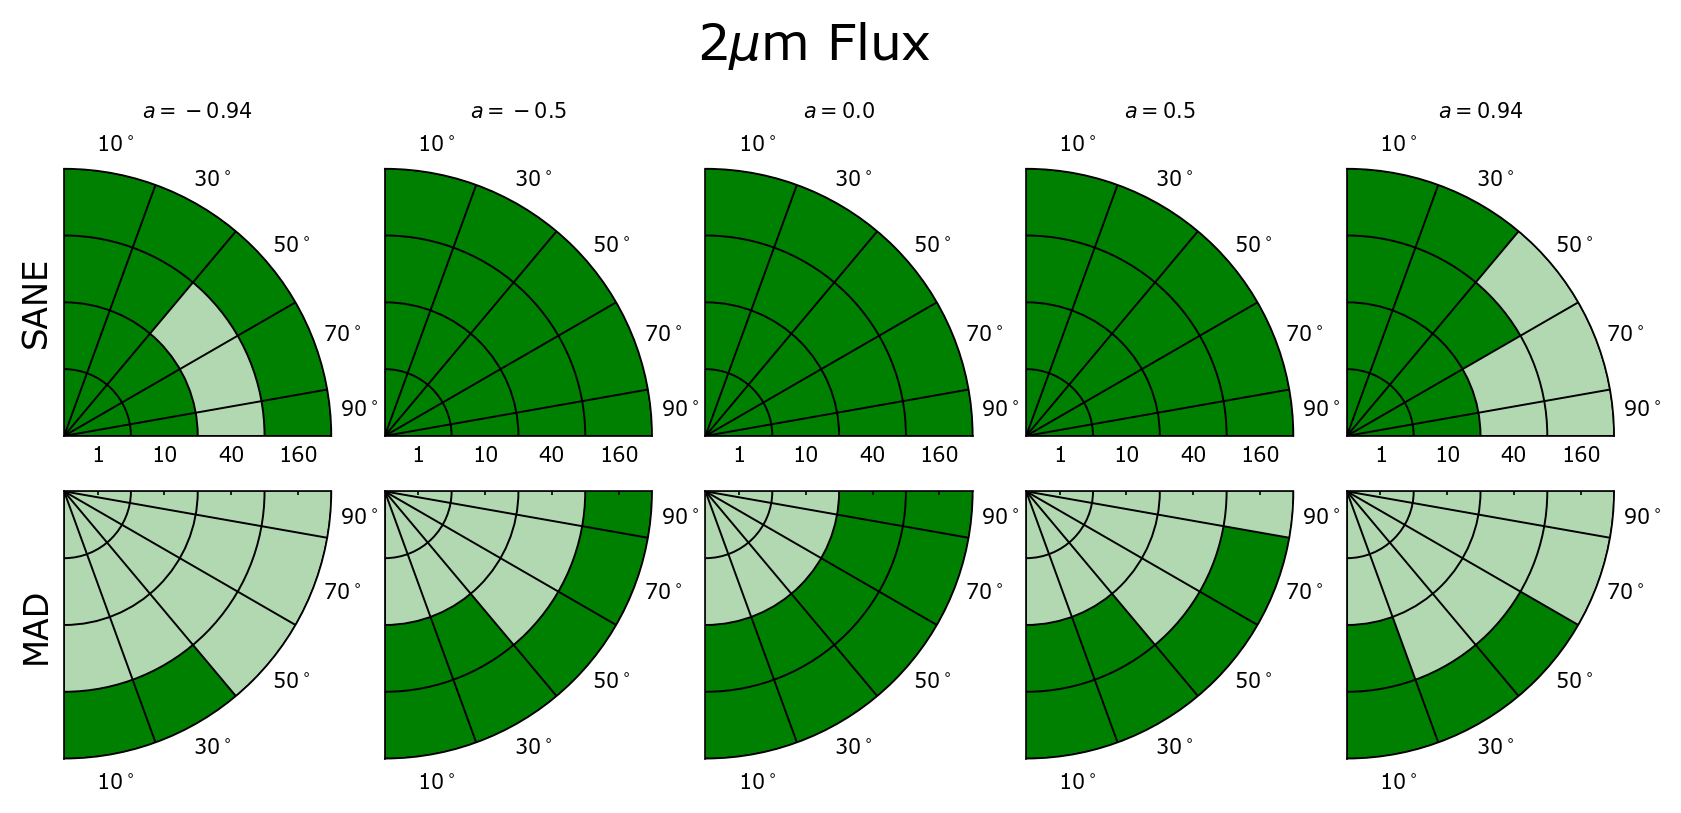
\includegraphics[width=\columnwidth]{./figures/2um_flux.png}
  \caption{NIR flux limit}
  \label{fig:cmp_2um_flux}
\end{figure}

[Michi]

%..............................................................................
\subsubsubsection{X-ray Luminosity}

[George to provide physical overview]

Estimates of flux from Compton.

Estimates of Bremss.  Discussion of Bremss. in SANE, large Rhigh models.

\begin{figure}
  \centering
  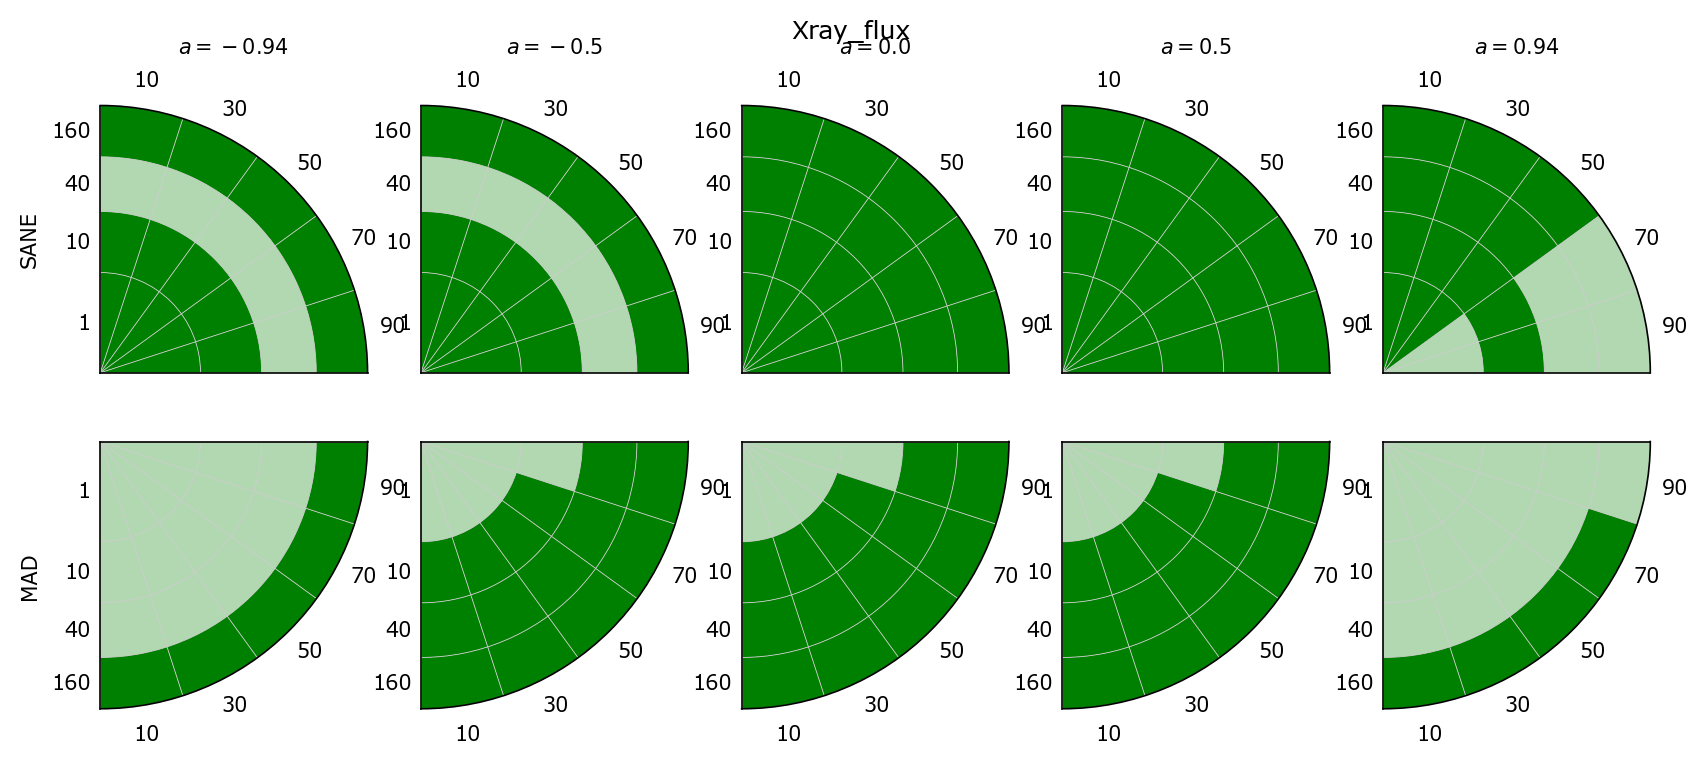
\includegraphics[width=\columnwidth]{./figures/Xray_flux.png}
  \caption{X-ray flux limits}
  \label{fig:cmp_xray_flux}
\end{figure}

[Michi]

%..............................................................................
\subsubsubsection{86 GHz Median Flux}

\begin{figure}
  \centering
  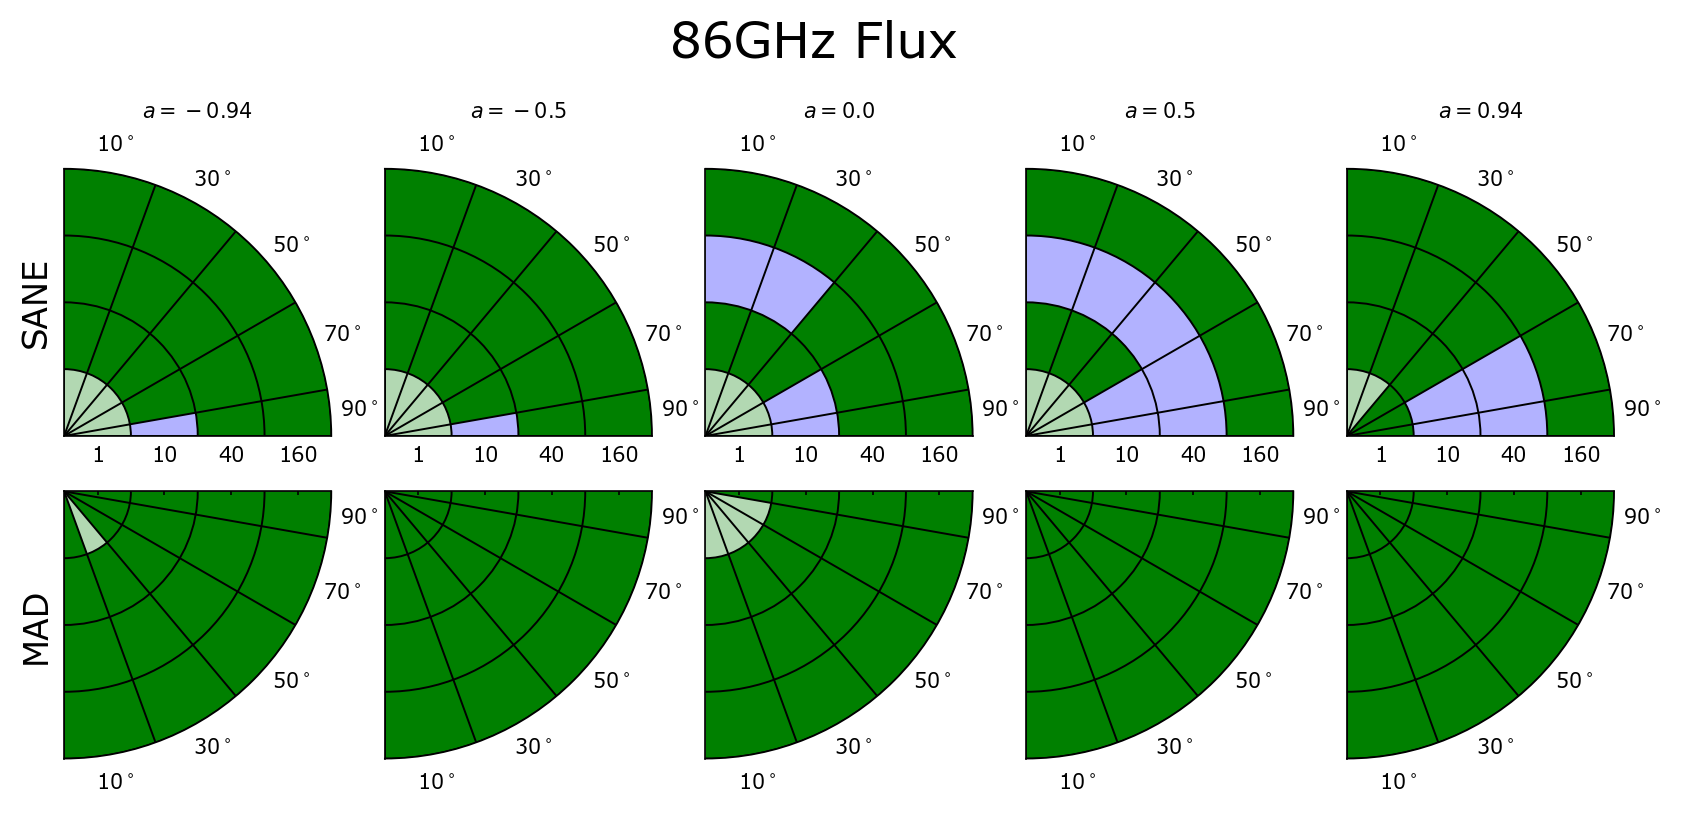
\includegraphics[width=\columnwidth]{./figures/86GHz_flux.png}
  \caption{86GHz median flux limits}
  \label{fig:cmp_86ghz_flux}
\end{figure}

[Michi]

%..............................................................................
\subsubsubsection{86 GHz Major Axis}

\begin{figure}
  \centering
  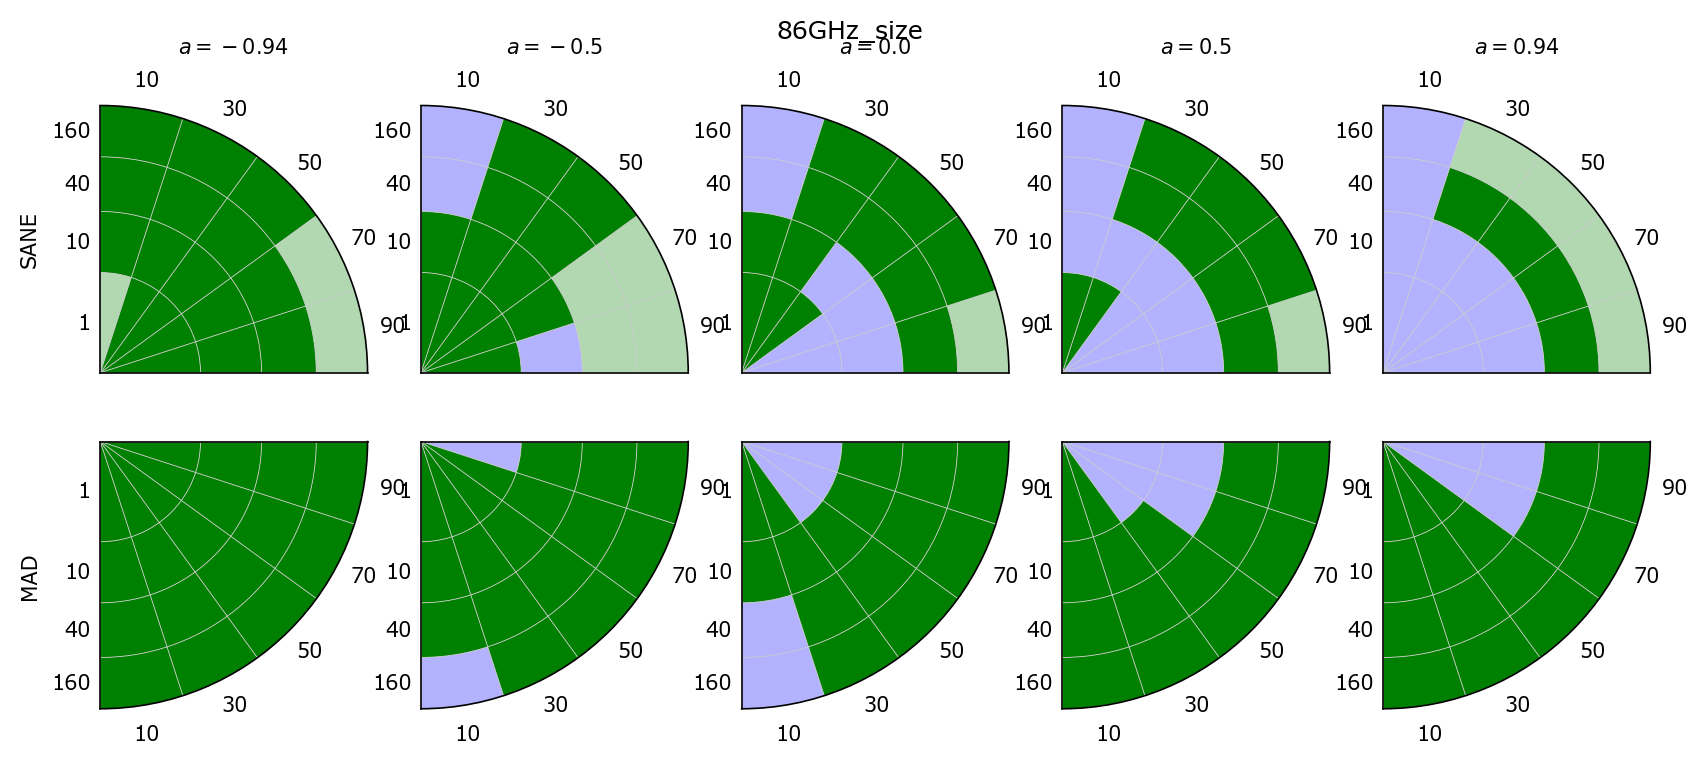
\includegraphics[width=\columnwidth]{./figures/86GHz_size.png}
  \caption{86GHz size}
  \label{fig:cmp_86ghz_size}
\end{figure}

[Michi]

\subsubsubsection{Summary of Non-EHT constraints}

\begin{figure}
  \centering
  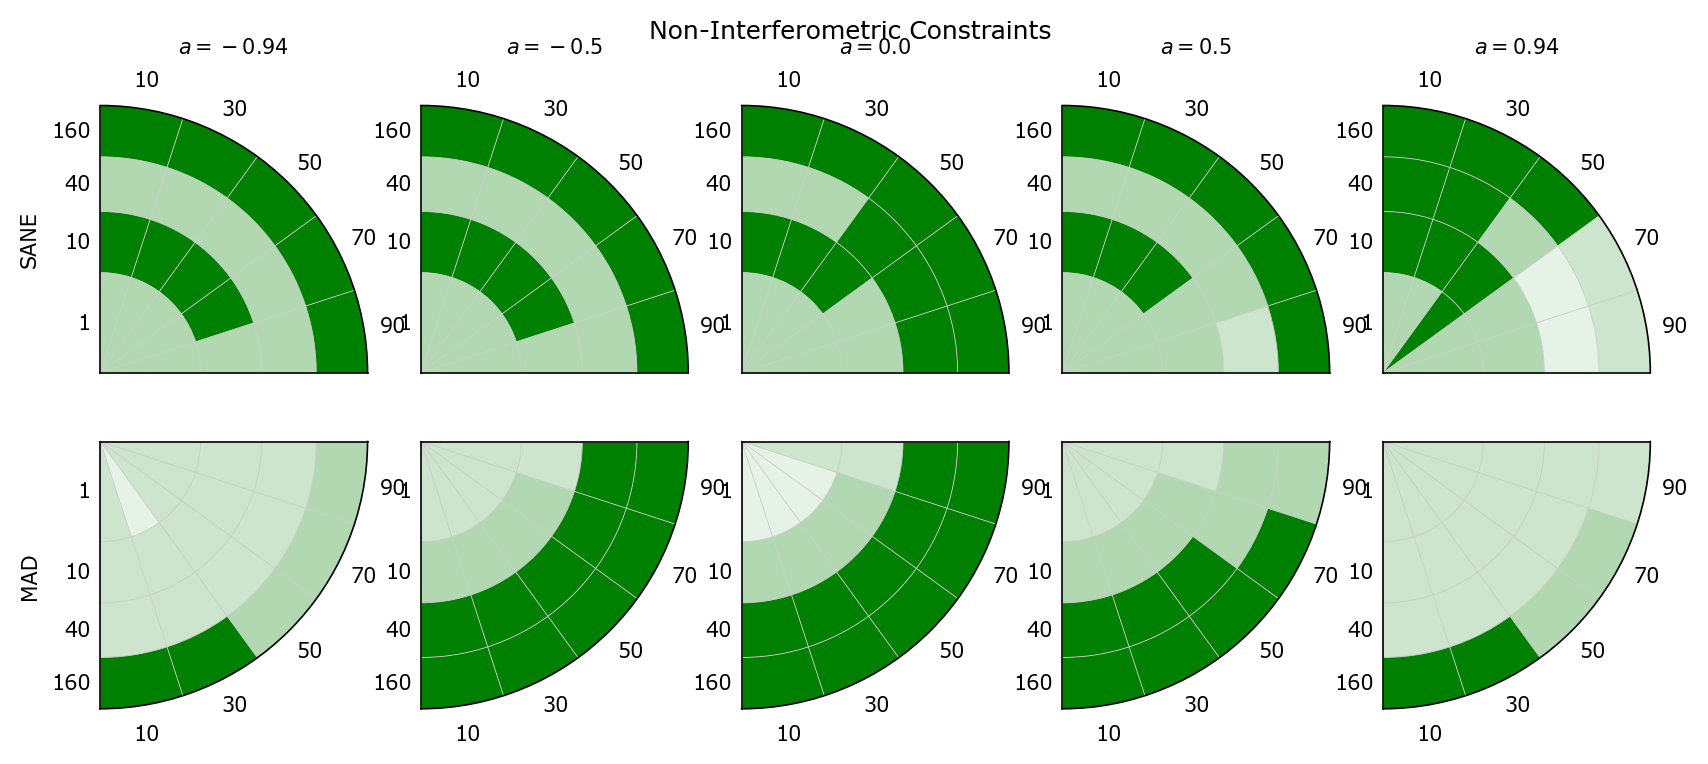
\includegraphics[width=\columnwidth]{./figures/Noninterferometric_Hard_Cut.png}
  \caption{Combined non-EHT constraints}
  \label{fig:non_eht_cuts}
\end{figure}

\subsubsection{Summary of All Constraints}

\begin{figure}
  \centering
  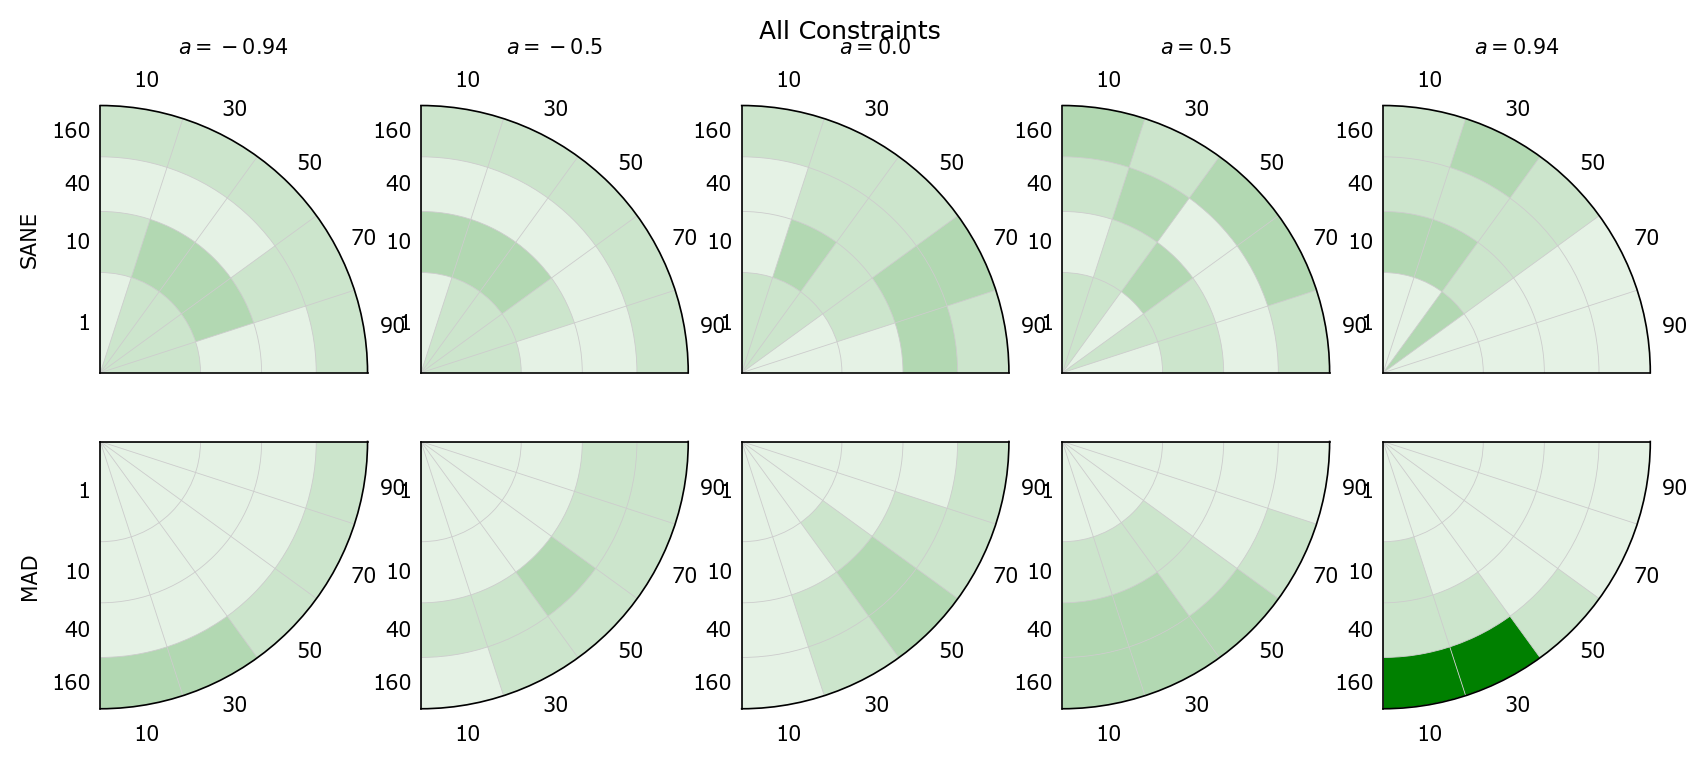
\includegraphics[width=\columnwidth]{./figures/All_Hard_Cut.png}
  \caption{Combined EHT and non-EHT constraints}
  \label{fig:all_cuts}
\end{figure}

\subsubsection{Inter-Model Comparison}


[Doosoo, Koushik to write here about HAMR thermal models.  Define a subsection, describe the results.]

[Angelo and Richard to write here about critical beta models.  Define a subsection, describe the results.]




%==============================================================================
\subsection{Nonthermal Aligned Models}

[Koushik to write here about powerlaw nonthermal HAMR models.  Define a subsection, describe the results and how they differ from the thermal results.][Maybe add Tomohisa's models here as well.] [by including power-law, we see this and that change (only include significant changes from the thermal models)]

[Razi to write here about variable kappa models.  Define a subsection, describe the results and how they differ from the thermal results.]

[Christian to write here about constant kappa models.  Define a subsection, describe the results and how they differ from the thermal results.]
\subsection{Constant kappa models $\kappa=3.5$ with variable efficiency, $\varepsilon(\sigma,\beta)$}

In order to investigate the fraction on thermal to non-thermal particles we combine a thermal electron distribution function with a kappa electron distribution with $\kappa=3.5$. The value of $\kappa=3.5$ is motivated from the spectral slope in the NIR during a quiescent state \cmf{add reference here}. In addition to the fixed kappa value we assume that the fraction between thermal and non-thermal particles depends on the local plasma properties, e.g, the magnetisation, $\sigma$, and the plasma beta parameter, $\beta_{\rm p}$. Given this assumption we can write the total emissivity as:
\begin{equation}
j_{\nu,\rm{tot}}=\left[1-\epsilon(\varepsilon,\beta, \sigma)\right] j_{\nu,\rm{thermal}} + \epsilon(\varepsilon,\beta, \sigma) j_{\nu, \kappa},
\label{eq:kappaeff}
\end{equation}
where the efficiency, $\epsilon(\varepsilon,\beta,\sigma)$, is given by:
\begin{equation}
    \epsilon(\varepsilon,\beta,\sigma)=\varepsilon\left[] 1 - \exp\left(-\beta_{\rm p}^{-2}\right)\right]\left[1-\exp\left(\frac{-\sigma^2}{\sigma_{\rm min}^2}\right)\right].
\end{equation}
Throughout this work we fix $\sigma_{\rm min}=0.01$ and vary the base efficiency, $\varepsilon$, between 0.05, 0.1 and 0.2. For each base efficiency we generate a set of models spanning the same parameter space as the thermal models (see Table \ref{tab:radiativemodels} for details). For each model we iterate the mass accretion rate to obtain an average flux of 2.4\,Jy at 230\,GHz across a time interval of 5000\,M. In order to explore a several values of $\varepsilon$ we increased the cadence of the radiative transfer to 50\,M. This allows us to keep the numerical costs for this parameter sweep low while still being within the correlation time of the GRMHD simulations ($t_{\rm corr}\approx 50-100\,M$) \cmf{ do we have reference for this? So far this result is not published, maybe Boris paper?}. An example for the distribution of the efficiency can be seen in the right half of  Fig. \ref{fig:varepsilon}. The efficiency quickly approaches $\epsilon=0$ within the disk region while within the jet the efficiency reaches the defined base-efficiency. Thus, togehter with the used cut of in sigma, $\sigma_{\rm cut}=1$ the non-thermal particles are mainly located in jet sheath.

\begin{figure}
  \centering
    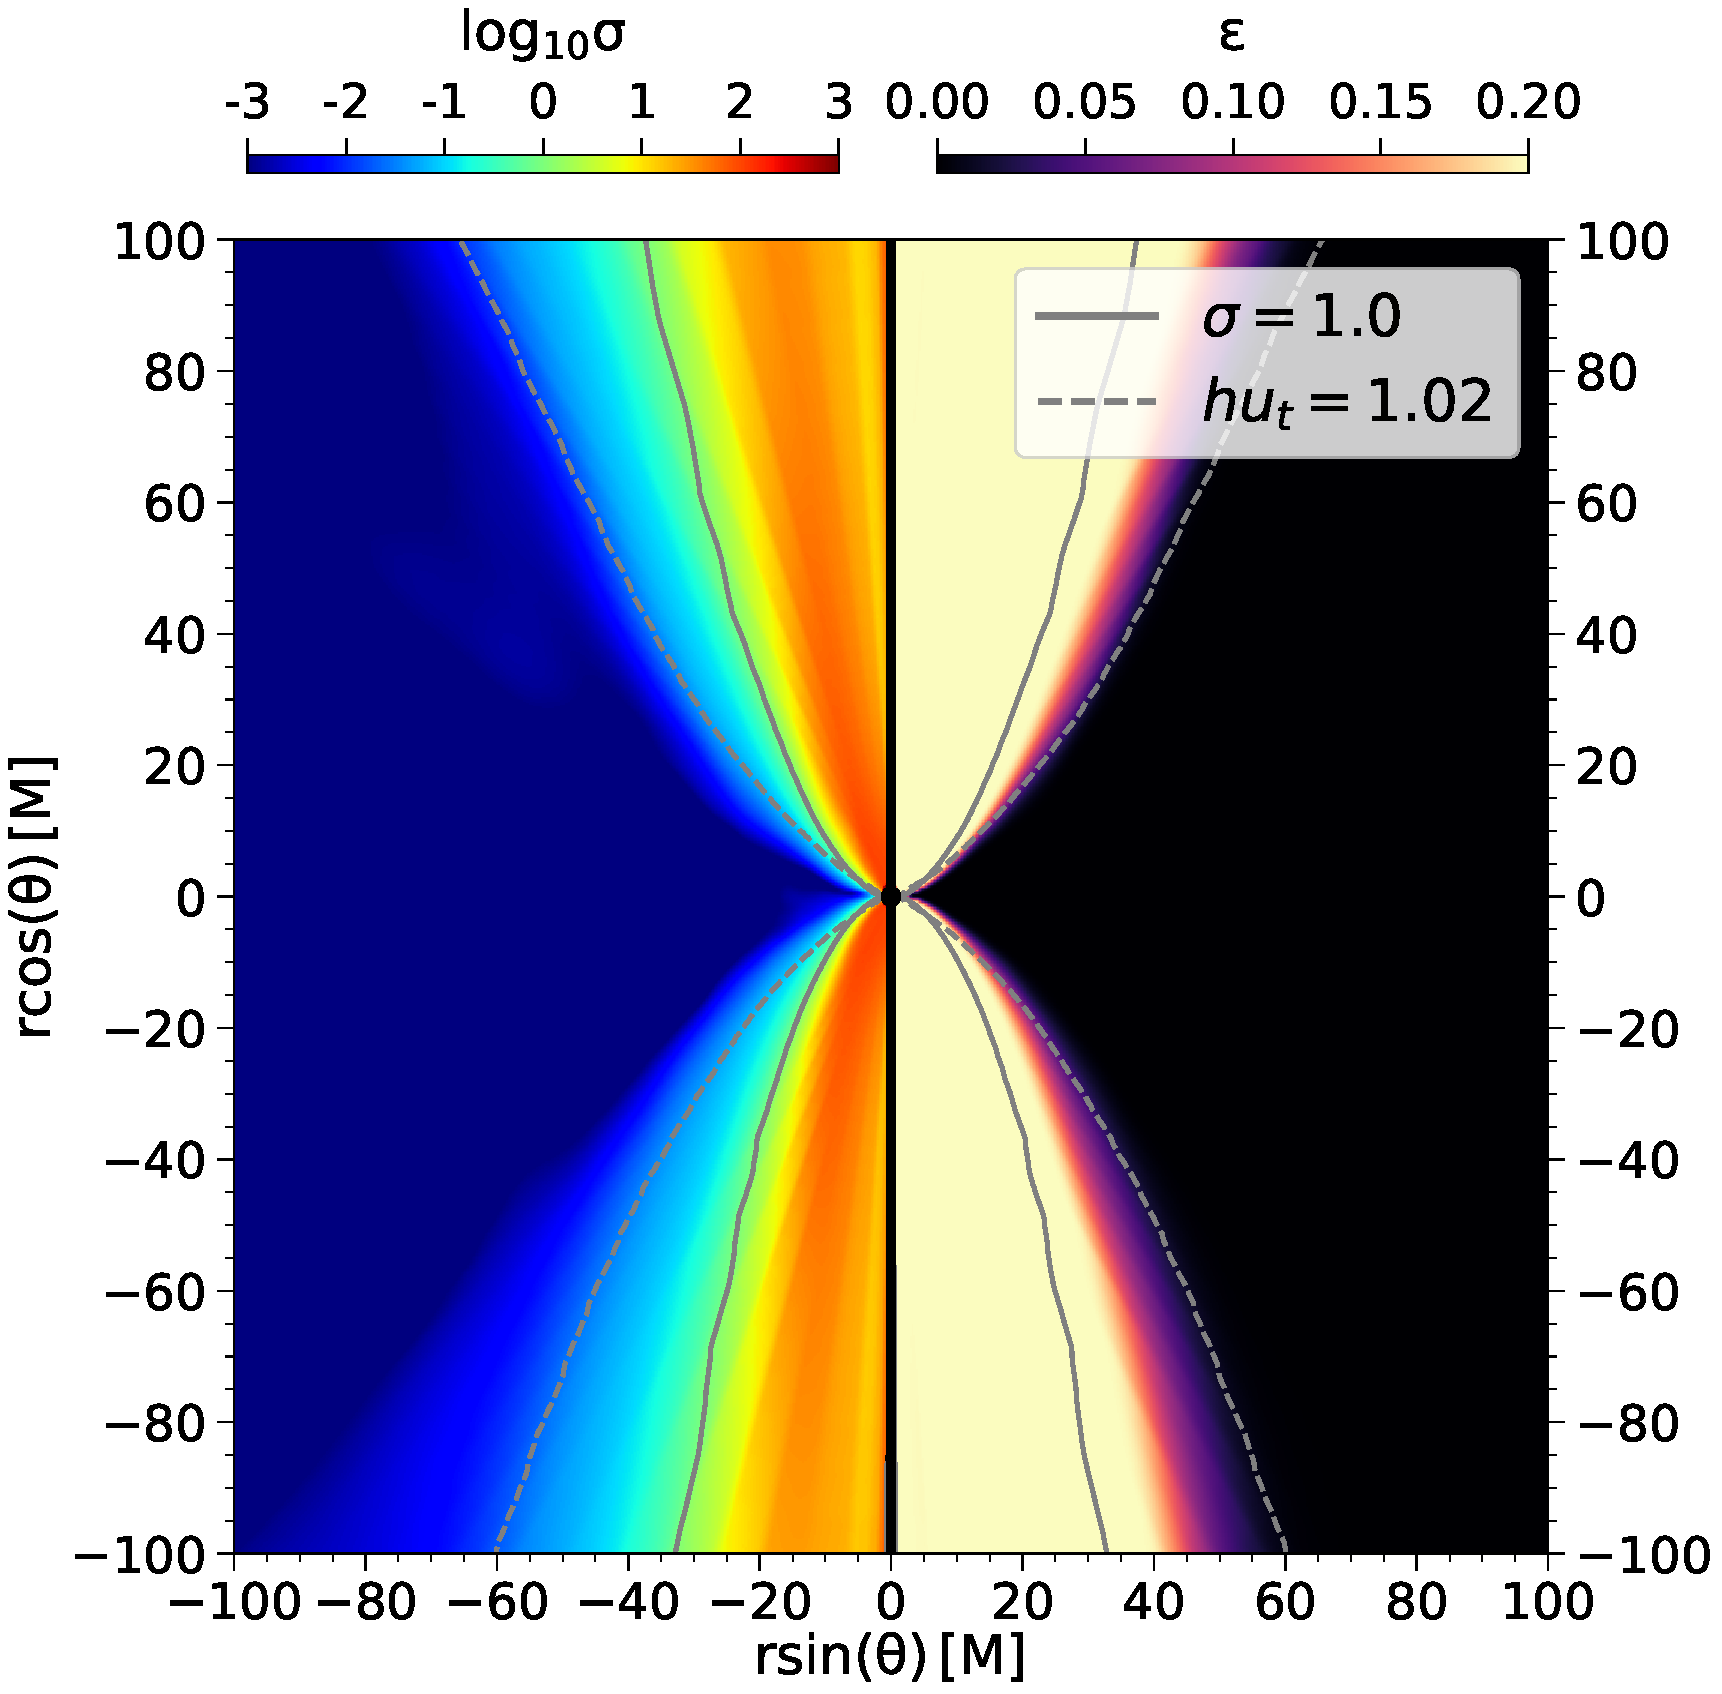
\includegraphics[width=\columnwidth]{./figures/GRMHDphiavera0.94sigmaeta.pdf}
  \caption{Time and azimuthal averaged distribution of the magnetization, $\sigma$ (left half) and the efficiency, $\epsilon(\varepsilon,\beta,\sigma)$ using $\varepsilon=0.2 $ for a BHAC MAD GRMHD simulation with spin $a_{\star}=0.94$. The solid gray line corresponds to $\sigma=1$ and the dashed line indicates out-flowing plasma vi the Bernoulli parameter ($-h u_{t}>1.02$).}
  \label{fig:varepsilon}
\end{figure}

In the following we will elaborate the impact of adding non-thermal particles via the kappa electron distribution with fixed kappa value ($\kappa=3.5$) and there different base efficiencies $\varepsilon=$0.05, 0.1 and 0.2 on the observational constraints listed in Sect. \ref{}.

\subsubsection{230\,GHz VLBI pre-image size} 
The addition of non-thermal particles alters the 230\,GHz VLBI pre-image sizes hardly for the MAD models and shows a minor effect on the SANE models. In the SANE case only models with $R_{\rm high}>40$ exhibit a minor increase in the source size where we see a monotonic increase of the source size with inclination. This effect can be understood if we consider that the bulk of the emission in all cases consider here is still produce by the thermal electron distribution, their temperature is given by Eq. \ref{} and an increase in $R_{\rm high}$ suppresses the emission from particles in the disk (by decreasing the electron temperature) and thus enhances the emission from jet. 
Given that most the non-thermal particles are located in the sheath of the jet their impact on the source size is largest if bulk of the thermal emission is also produced there. In addition the emissivity of thermal synchrotron radiation decreases as $j_{\nu}\propto \exp{\left(-\nu^{1/3}
\right)}$ while for the kappa distribution as $j_{\nu}\propto \nu^{-(\kappa -2)/2}$. This implies that for the same electron temperature the non-thermal flux is compared to a thermal one higher and thus leads to a more extended jet structure for the models including non-thermal particles.
\newline In the MAD case, independent of the choice of $R_{\rm high}$ the emission is mostly produced in the disk region (see EHT paper V and Fig 8 in Wong et al. 2021 for 3D rendering). Increasing $R_{\rm high}$ will not push the emission region into the jet where the non-thermal particles are located and thus their contribution to the total emission structure is negligible. 


\subsubsection{86\,GHz flux}
Since the GMVA+ALMA observations at 86\,GHz \cmf{ref to Issaoun paper} probe a larger field of view as the 230\,GHz EHT observations, we increased the field of view for the 86\,GHz to 800\,$\rm{\mu as}$ during the radiative transfer calculations. As mentioned earlier the non-thermal particles are mainly located in the jet sheath and thus the increased field of view ensures that no extend flux is missing during the comparison with the 86\,GHz observations.
\newline The 86\,GHz for both SANE and MAD models flux is not affected by the addition of non-thermal particles. In case of the SANE models the edges of the 86\,GHz flux distribution are slightly shifted in the case of $R_{\rm high}>40$. However, including non-thermal particles even with the highest base efficiency $\varepsilon=0.2$ does not change the scoring of a model, i.e., a thermal-only model which full-fills the 86\,GHz constrain is still accepted if non-thermal particles are included. This behaviour can be explained by the fact that the bulk of the emission in both accretion models is generated in with a few gravitational radii. Since the non-thermal particles are mainly located in the jet sheath and thei ratio between non-thermal to thermal particles is at most 20\% the contribution of the non-thermal particles to the 86\,GHz flux can be neglected.


\subsubsection{86\,GHz image size}
The behaviour of the 86\,GHz image size is very similar to the above described 230\,GHz image size: There is no change in image size for the MAD models and only a minor increase in the SANE models for $R_{\rm high}>40$. The physical reasons for this behaviour follows the same arguments as in the 230\,GHz VLBI pre-image size.

\subsubsection{NIR constraints}
As expected, the addition of non-thermal particles via the kappa electron distribution function with variable efficiency has a large influence on the NIR flux for all models independent of the accretion model and the $R_{\rm high}$ value. In Fig.~\ref{fig:NIR_kappaepsilon} we compare the distribution of the NIR fluxes for thermal and kappa eDF for a SANE accretion model.


\begin{figure}
  \centering
  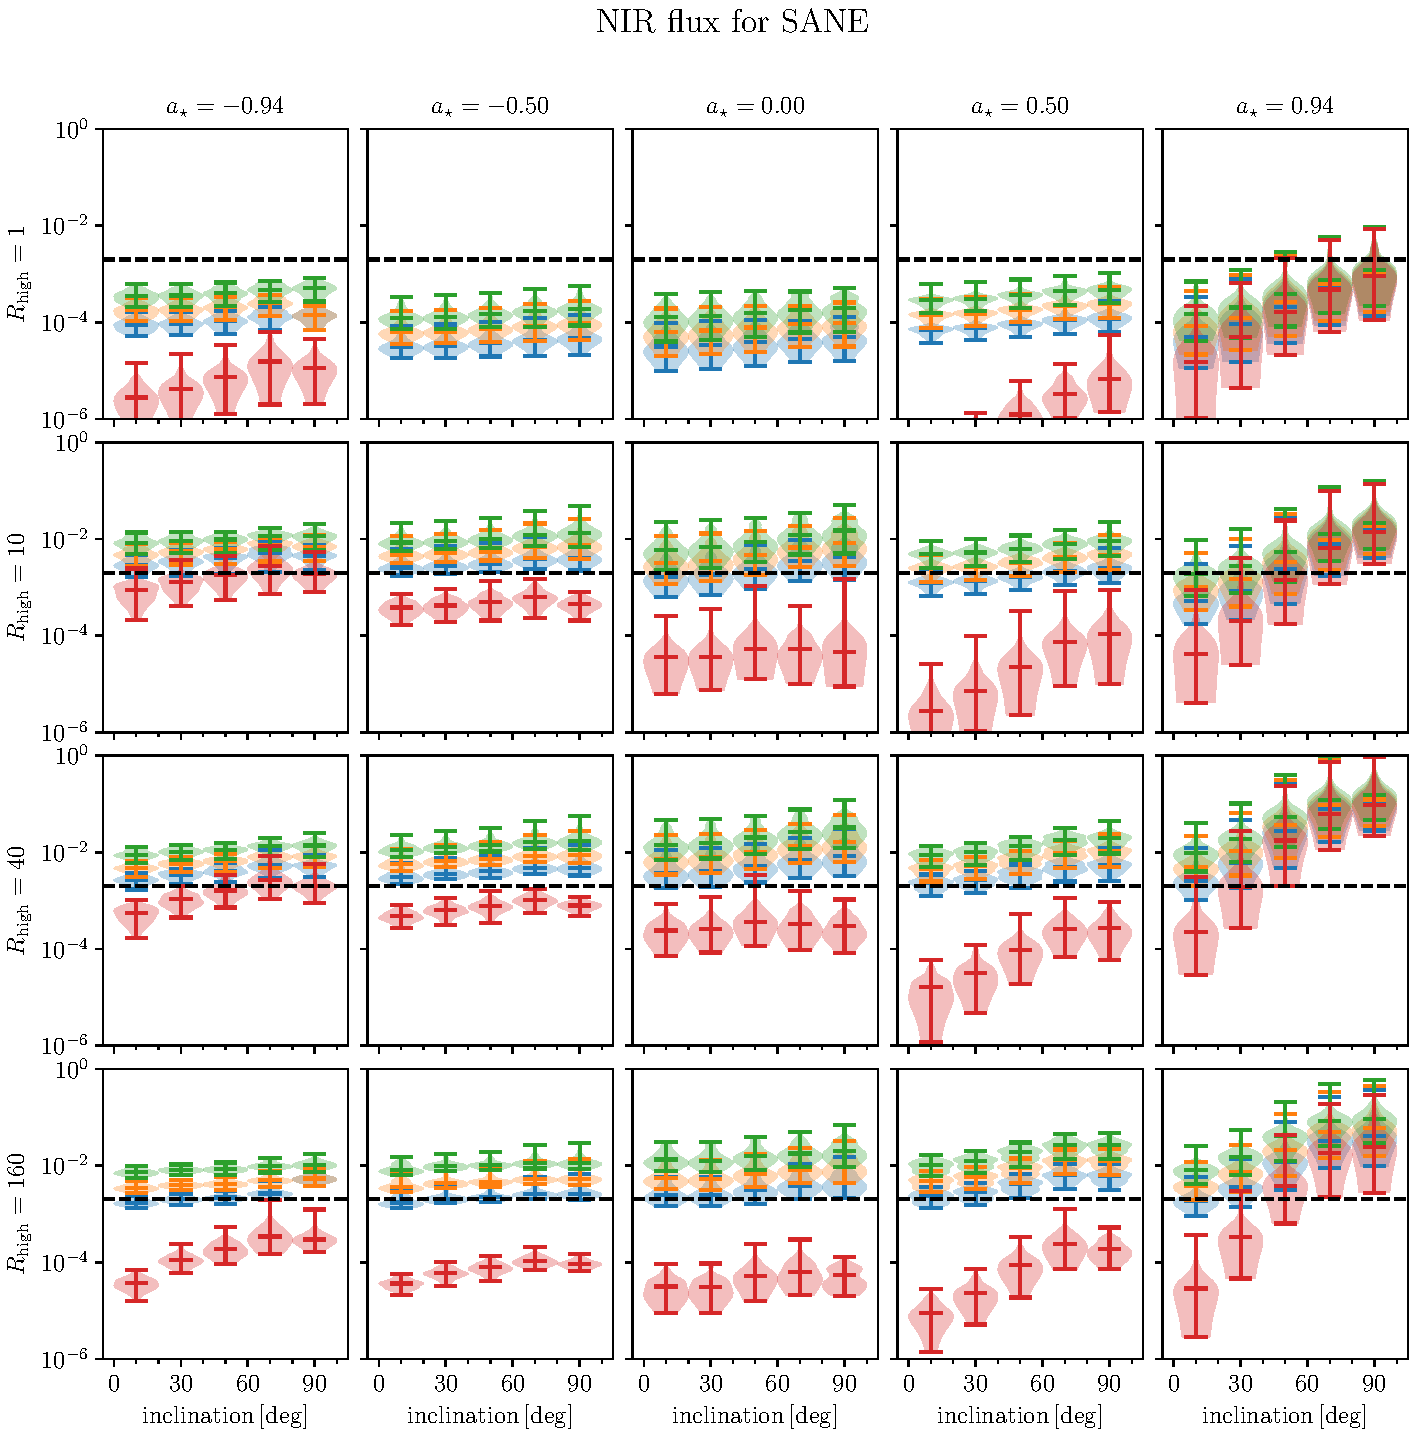
\includegraphics[width=\columnwidth]{./figures/SANE_NIR_standard.pdf}
  \caption{NIR constraints for SANE accretion models for thermal and non-thermal electron distribution function with $\kappa=3.4$ fixed and $\epsilon\left(\sigma,\beta,\varepsilon\right)$. The red violin plots correspond to a thermal eDF, blue, orange and green indicate kappa eDF with $\varepsilon=$0.05,0.1 and 0.2.}
  \label{fig:NIR_kappaepsilon}
\end{figure}

As can be seen in the figure, including non-thermal particles changes the distribution of the NIR fluxes significantly. Except for the $R_{\rm high}=1$ models the addition of non-thermal particles even with the lowest base efficiency used in this analysis $\left( \varepsilon=0.05\right)$ leads to a over-production of NIR fluxes. In the case of the MAD models all models over-produce the NIR flux for $\varepsilon=0.05$. 
\newline The NIR fluxes are produced by particles in the tail of the distribution function and are therefore are sensitive to slope of the tail. The emissivity for a thermal distribution decreases exponentially $\left(j_{\nu}\propto\exp(-\nu^{1/3})\right)$ while for the kappa distribution it behaves like $j_{\nu}\propto \nu^{-(\kappa-2)/2}$. Thus even at low base efficiencies, $\varepsilon$, the the flux from the kappa distribution in the NIR $\left(\nu\sim 10^{14}\,\rm{Hz}\right)$ is larger than for the thermal eDF.

\subsubsection{ALMA Light curves}
For the comparison with the ALMA light curves we compute the modulation index for a 3\,hour time window and across the entire simulated time window of 28\,hours (5000\,GM/c$^3$). Similar to the 86\,GHz flux the 230\,GHz flux is mainly produced within a few gravitational radii and thus not affected by the addition of non-thermal particles using Eq. \ref{eq:kappaeff}. As in the previous constraints, the MAD accretion models are insensitive to the addition of non-thermal particles whereas the SANE models show some increased modulation index for $R_{\rm high}>40$. However, the distributions for thermal and non-thermal eDF are still largely overlapping. 


\subsubsection{Conclusions}
The effect of adding non-thermal particles via a kappa electron distribution function with fixed $kappa=3.4$ values and 
[Alejandro to write here about Frankfurt nonthermal models.  Define a subsection, describe the results and how they differ from the thermal results.]

[Tomohisa to write here about UWABAMI nonthermal power-law models]

\ckc{Write subsections only if they are different from the thermal models.}


\subsection{Variable kappa model}
...  


%==============================================================================
\subsection{Tilted Models}

[Koushik to write here.  Describe the results and how they differ from aligned thermal results.]

\ckc{Write subsections only if they are different from the thermal models.}

%==============================================================================
\subsection{Stellar Wind Fed Models}

[Angelo and George to write here.  Describe the results and how they differ from aligned thermal results.]

\ckc{Write subsections only if they are different from the thermal models.}

%==============================================================================
\subsection{Best Bet Models}

\begin{figure*}
    \centering
    [altex: a grid figure showing the $\sim$ 4 best bet models.  Each model in a column.  Top two rows are the 230GHz images and 86GHz images, last row is SEDs.]
    \caption{Best bet models.  Each column corresponds to one best bet model; top row shows a 230GHz image [average or selected image; or use GIF?]; middle row shows an 86GHz images; bottom row shows SEDs.}
    \label{fig:my_label}
\end{figure*}

[Michi to provide first draft]

We now consider combined constraints, excluding variability, under the hypothesis that (1) there is a missing physical ingredient in the models that would lower variability, but (2) that missing ingredient would not vitiate the models entirely.  Models are eliminated if they fail any one constraint.

Figure showing combined constraints for thermal models.

Figure showing combined constraints for nonthermal models.

We then inspected the remaining models and selected four best-bet models that approximately span the space of successful models.  [Written characterization of remaining models; possibly 3 or 5].
